
\textbf{\underline{Вторая глава}} раскрывает решения трех оптимизационных задач, связанных с оптимизацией конструкции робота.

\textbf{Первая задача:} оптимизировать количество ног у объекта исследования на основе критериев, представленных ниже \pic{fig:opti_criteria}. 

\begin{figure}[H]
    \begin{subfigure}{0.49\textwidth}
        \centering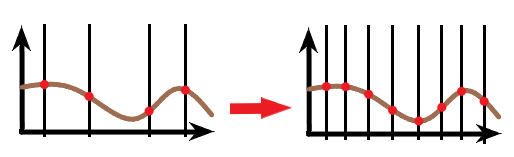
\includegraphics[height=6cm,width=1\textwidth,keepaspectratio]{f1.png}
        \caption{При увеличении количества ног увеличивается детализация картографируемой поверхности}
        \label{fig:f1.png}
    \end{subfigure}
    \begin{subfigure}{0.49\textwidth}
        \centering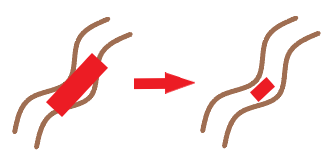
\includegraphics[height=6cm,width=1\textwidth,keepaspectratio]{f2.png}
        \caption{При увеличении количества ног, корпус робота увеличивается и он не может пройти часть препятствий}
        \label{fig:f2.png}
    \end{subfigure}

    \hfill
    \begin{subfigure}{\textwidth}
        \centering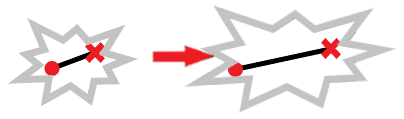
\includegraphics[height=2cm,width=1\textwidth,keepaspectratio]{f3.png}
        \caption{При изменении количества ног меняется проходимость системы}
        \label{fig:f3.png}
    \end{subfigure}
    \hfill

\caption{Критерии оптимизации конструкции робота}
\label{fig:opti_criteria}
\end{figure}
Чем больше количество полученных точек на пройденной поверхности, тем выше будет детализация карты. Одним из способов увеличения детализации это увеличение количества ног у робота \pic{fig:f1.png}. С другой стороны, это увеличивает длину робота, а следовательно робот хуже сможет проходить узкие участки с обилием поворотов \pic{fig:f2.png}. Чем большее расстояние робот сможет пройти за одно и то же время, тем быстрее будет построена карта и робот меньше повлияет на окружающую среду при прочих равных условиях \pic{fig:f3.png}. 

Для цикловых движителей с одной степенью свободы в ноге вопрос о количестве ног не имеет однозначного решения. Поэтому необходимо провести структурный синтез, чтобы определить их количество. Данная задача решалась с помощью генетического алгоритма.

Идея решения следующая. Генерируется семейства территорий (делается предположение, что территория, сгенерированная на основе одинаковых параметров является одинаково сложной \pic{fig:terrains}). Индивид запускается на фиксированное время на данную территорию, на моторы подается константная угловая скорость. Результаты пройденной дистанции и параметры робота записываются и участвуют в функции оптимизации.

\begin{figure}[h]
    \begin{subfigure}{0.33\textwidth}
    \centering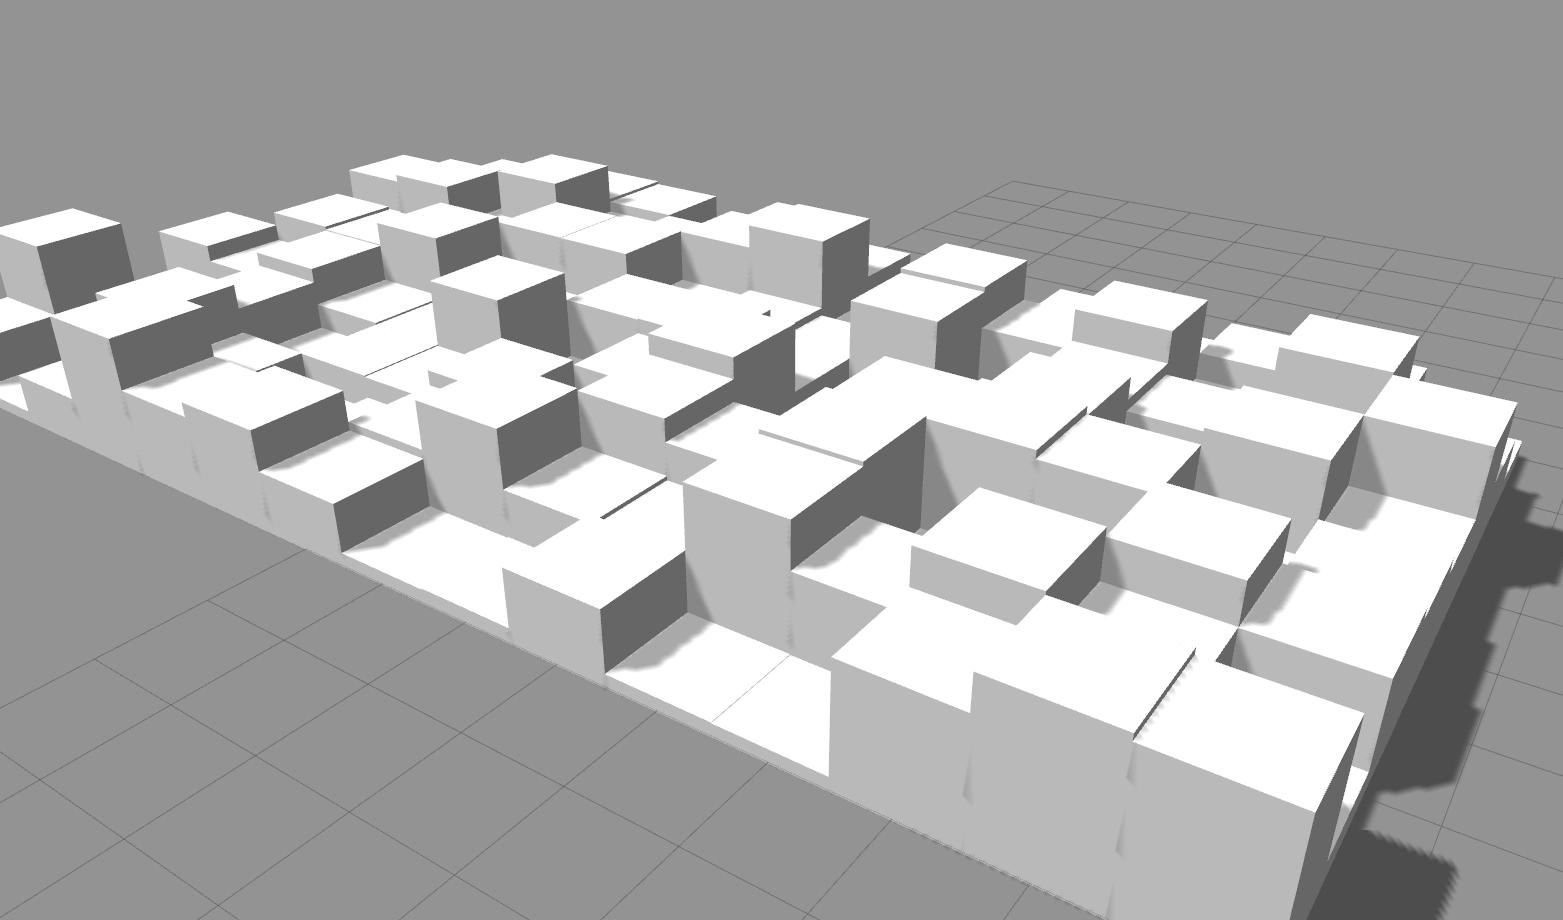
\includegraphics[width=0.8\textwidth]{terrain_1} 
    \caption{T1: 3D-боксы с равномерным распределением высоты}
    \label{fig:terrain_1}
    \end{subfigure}
    \begin{subfigure}{0.33\textwidth}
    \centering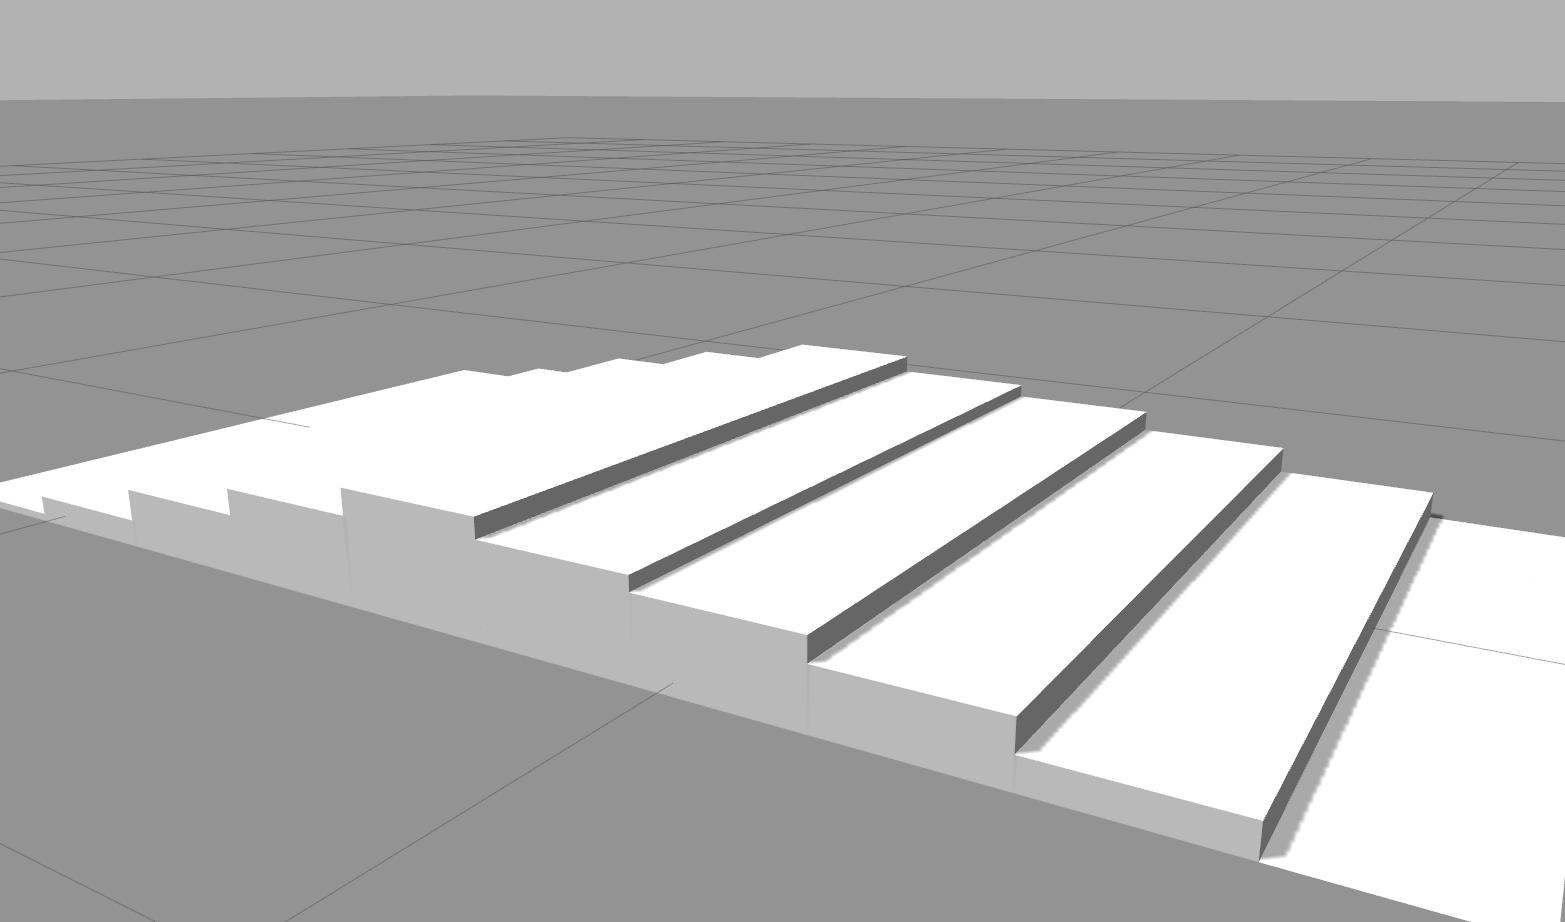
\includegraphics[width=0.8\textwidth]{terrain_2} 
    \caption{T2: 2D-полосы с гауссовой функциональной высотой}
    \label{fig:terrain_2}
    \end{subfigure}
    \begin{subfigure}{0.33\textwidth}
    \centering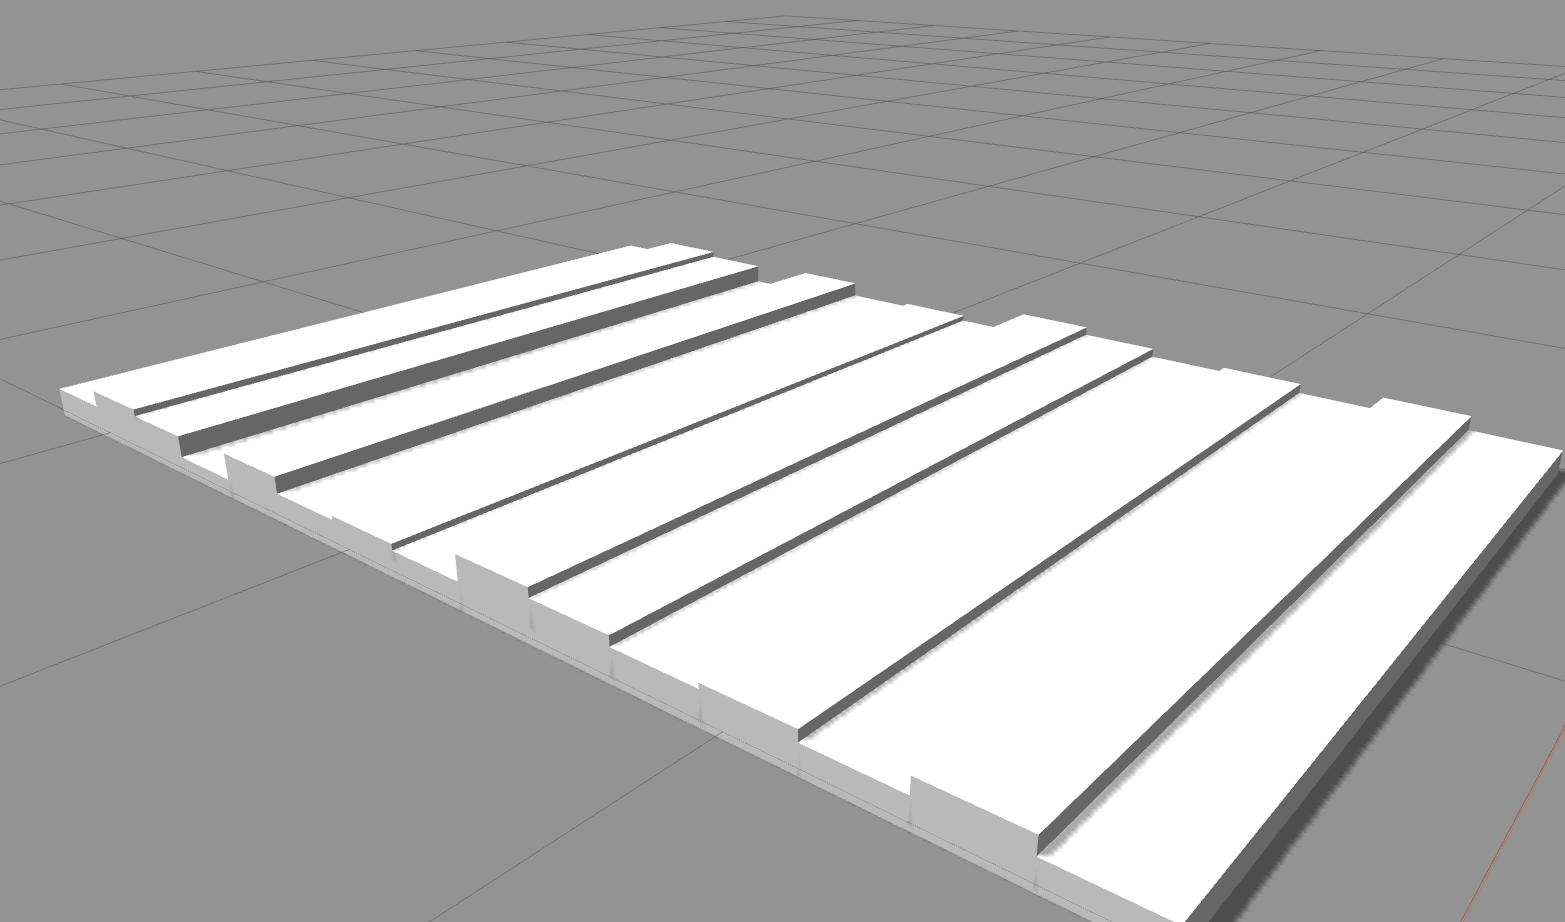
\includegraphics[width=0.8\textwidth]{terrain_3}
    \caption{T3: 2D-полосы с распределением высоты по гауссовой функции)}
    \label{fig:terrain_3}
    \end{subfigure}
     
    \caption{Примеры сгенерированных территорий}
    \label{fig:terrains}
\end{figure}

Для начала требуется описать математическую модель системы. Исследуется механическая система, состоящая из твёрдых тел \eqref{eq:newton_euler}, движение которых описывается дифференциальными уравнениями вида:

\begin{align}
    \label{eq:newton_euler}
    M \dot{\vec{u}} = \vec{g} \\
    M = \begin{bmatrix}
    M_1 & \cdots  & 0 \\
    \vdots  & \ddots  & \vdots  \\ 
    0 & \cdots   & M_n 
    \end{bmatrix},\ M_i = \begin{bmatrix}
    m_i E_{3\times 3} & 0 \\ 
    0 & I_i 
    \end{bmatrix} \\
    \vec{u}_i^{\ T} = \begin{bmatrix}
        \vec{v}_i^{\ T} & \vec{\omega}_i^{\ T}
    \end{bmatrix} \\ 
    \vec{g}^{\ T} = \begin{bmatrix}
        \cdots \  \vec{F}_i^{\ T}, & (\vec{\tau}_i - \vec{\omega}_i \times I_i \vec{\omega}_i)^T\  \cdots 
    \end{bmatrix}
\end{align}
где, $M_i$ --- матрицы, содержащие массово-инерционные характеристики; $m_i$ масса тела; $I_i$ тензор инерции; $\vec{u_i}$ вектор обобщённых скоростей; $E$ --- единичная матрица; $\vec{g}$ вектор обобщённых сил; $\vec{v_i}$ вектор линейной скорости; $\vec{\omega_i}$ --- вектор угловой скорости; $\vec{F_i}$, $\vec{\tau_i}$ силы и моменты сил взаимодействия.

Тела, входящие в систему соединены между собой цилиндрическими шарнирами, которые описываются следующими связями и динамическими ограничениями \eqref{eq:kin_constr}:
\begin{align}
    \label{eq:kin_constr}
    \phi(q_{j_1},\ u_{j_1},\ \cdots,\ q_{j_k},\ u_{j_k},\ t) \geqslant  0 \\
    \vec{q_i}^{\ T} = \begin{bmatrix}
        \vec{x}_i^{\ T} & \vec{Q}_i^{\ T}
    \end{bmatrix} \\
    \dot{\vec{q_i}} = \begin{bmatrix}
    E_{3\times3} & 0\\ 
    0 & G(\vec{q}_i) 
    \end{bmatrix}\vec{u}_i  \\
    \vec{g}_i = \tau_i^T \vec{z}_{i-1} -k_i \dot{\vec{q_i}}
\end{align}
где через $\phi$ обозначена функция связи; $t$ время; $q_{j}$ --- вектор обобщенных координат, включающий в себя координаты центра масс $\vec{x_i}$ и кватернион $\vec{Q_i}$, описывающий ориентацию тела в пространстве; через $G(\vec{q}_i)$ обозначена матрица, вид которой зависит от выбранной системы координат и способа задания ориентации тела; $k$~---~ коэффициент вязкого трения в шарнире.

Контакт ног робота с опорной поверхностью \pic{fig:contact_interaction.png} описывается на базе модели сухого трения и выражается следующими уравнениями \eqref{eq:contact_inter}:


\begin{align}
    \label{eq:contact_inter}
    \phi_u(\vec{q}\ ) \geqslant 0 \\ 
                        \phi_u(\vec{q}\ ) = (\vec{x}_1 + \vec{s}_1 - \vec{x}_2 - \vec{s}_2) \cdot \vec{n} \\
                        \frac{d }{d t}\phi_u(\vec{q}\ ) \approx \begin{bmatrix}
                            \vec{n}^{\ T} & (\vec{s}_1 \times \vec{n})^T & -\vec{n}^{\ T} & (-\vec{s}_2 \times \vec{n})^T
                        \end{bmatrix} \begin{bmatrix}
                            \vec{v}_1\\ 
                        \vec{\omega}_1\\ 
                        \vec{v}_2\\
                        \vec{\omega}_2\\
                        \end{bmatrix} \\
\left\{\begin{matrix*}[l]
\mu f_n \geqslant \sqrt{f_1^2 + f_2^2}\\ 
\left\lVert \vec{v_t}\right\rVert (\mu f_n - \sqrt{f_1^2 + f_2^2}) = 0\\
\dfrac{\vec{f_t}}{\left\lVert \vec{f_t}\right\rVert } = - \dfrac{\vec{v_t}}{\left\lVert \vec{v_t}\right\rVert }
\end{matrix*}\right.
\end{align}
где, $\phi_u(\vec{q})$ --- функция связи; $\mu $ --- коэффициент трения между ногой и опорной поверхностью; $\vec{x}_{1,2},\ \vec{s}_{1,2}$ --- радиус-векторы и орты координатных осей $\vec{t}_{1,2}, \vec{n}$ показаны на рисунке \pic{fig:contact_interaction.png}; $ f_{1,2} $ --- значения сил трения вдоль осей $t_{1,2}$ соответственно.

\begin{figure}[H]
    \centering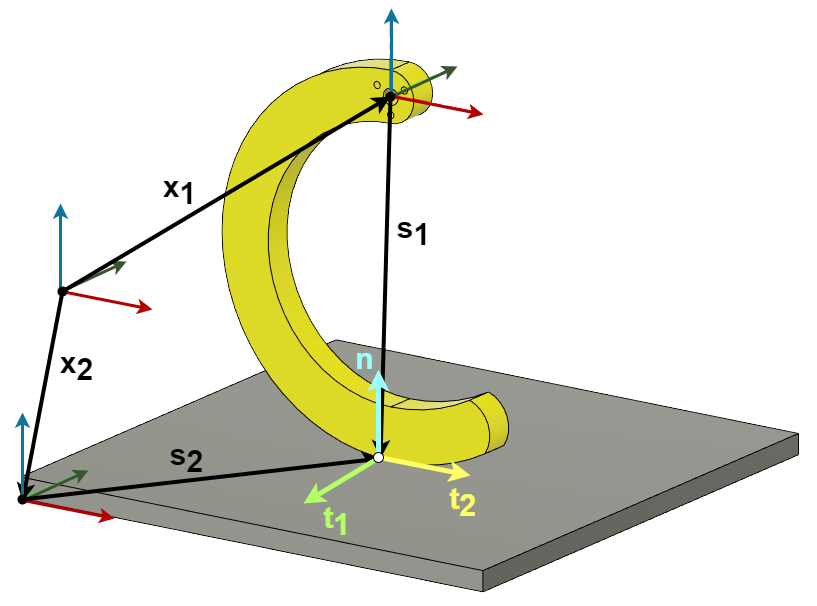
\includegraphics[height=3.9cm,width=1\textwidth,keepaspectratio]{images/contact_interaction.png}
    \caption{Отображение переменных для модели взаимодействия опорной поверхности и ноги робота}
    \label{fig:contact_interaction.png}
\end{figure}
Геометрическая модель робота представлена в виде трехмерного параллелепипеда. Количество движителей по каждому из бортов обозначается через $\gamma$. Разность фаз между соседними движителями обозначается через  $\alpha$ \pic{fig:best_gen_robot.jpg}.

\begin{figure}[H]
    \centering
    \begin{tikzpicture}
        % Include the image in a node
        \node [above right, inner sep=0] (image) at (0,0)
        {\centering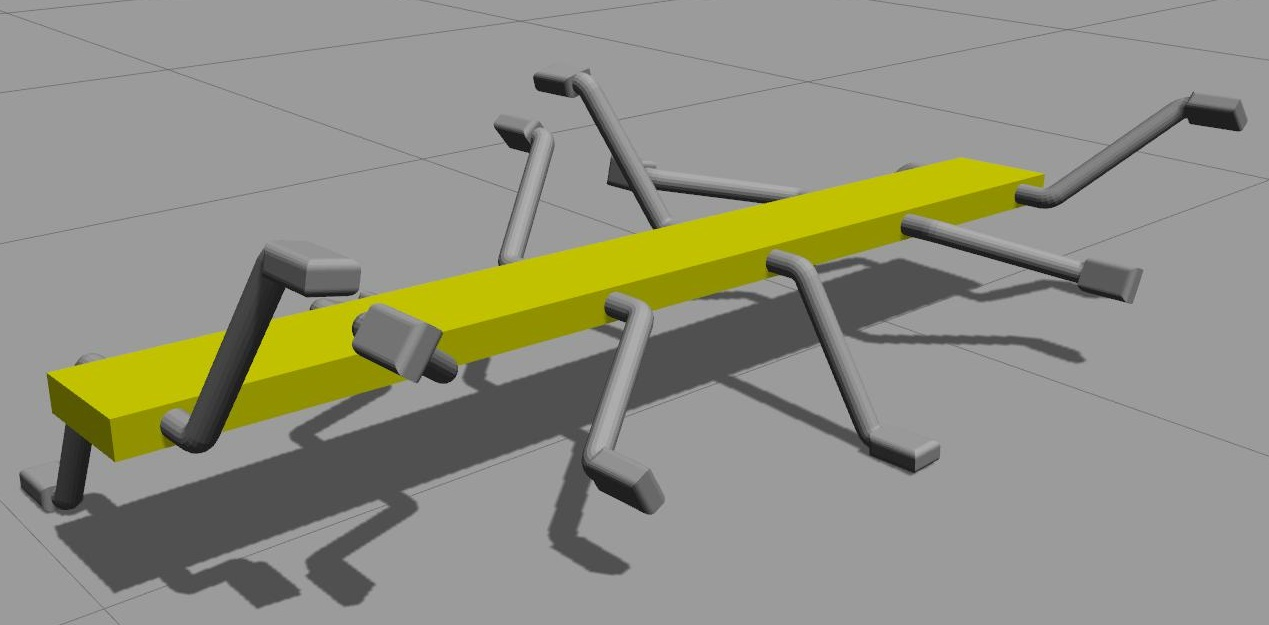
\includegraphics[height=2.7cm,width=1\textwidth,keepaspectratio]{best_gen_robot.jpg}};
        % Create scope with normalized axes
        \begin{scope}[
                x={($ 0.1*(image.south east)$)},
                y={($ 0.1*(image.north west)$)}]
            % Labels
            \draw [green, very thick,
                decorate,
                decoration = {brace,
                        raise=5pt,
                        amplitude=5pt,
                        aspect=0.5}] (1.4,3.6) --  (8.1,6.8)
            node[rounded corners=3pt, pos=0.5,above left =14pt,black,fill=white]{\tiny $(\gamma - 1) h_{\text{leg}}sin(\alpha)$};

            \draw[stealth-, very thick,green] (9.5,7.8) -- (7.8,1.94);
            \draw[stealth-, very thick,green] (1.5,2.8) -- (7,1)
            node[rounded corners=3pt,right,black,fill=white]{\tiny $\gamma = 6$};

            \draw[thin,green] (6.7,4) -- (5.75,9);
            \draw[thin,green] (4.85,3.5) -- (5.75,9);
            \draw[thin,green,stealth-stealth] (6.32,6) arc (-79.2:-99.2:3) node [rounded corners=3pt,below = 2pt,black,fill=white, midway] {\tiny $\alpha$};
        \end{scope}
    \end{tikzpicture}
    \caption{Схема модели робота для генетического алгоритма}
    \label{fig:best_gen_robot.jpg}
\end{figure}

Для решения задачи оптимизации нужно разработать целевую функцию. Так как количество ног и длина корпуса имеют прямую зависимость, то было решено решить мультикритериальную задачу оптимизации, где необходимо было максимизировать дистанцию, пройденную за фиксированное время, и минимизировать длину робота \eqref{eq:second}. Параметрами индивида являлись $\gamma$ и $\alpha$. Свертка осуществлялась с помощью мультипликативно-аддитивной свертки.

\begin{eqnarray}
    \label{eq:second}
    F \rightarrow max = \beta \left( {\omega}_{1} \cdot \overbrace{\delta}^{\text{Дистанция}} + {\omega}_{2} \cdot \overbrace{\frac{1}{(\gamma - 1) h_{\text{leg}}sin(\alpha)}}^{\text{Упр. длина тела}}\right) + \\ \nonumber + (1 - \beta) {\delta}^{{\omega}_{1}} {\left( \frac{1}{(\gamma - 1)h_{\text{leg}}sin(\alpha)}\right)}^{{\omega}_{2}}
\end{eqnarray}
где $\delta$ дистанция, $\beta$ адаптивный параметр, ${\omega}_{1,2} \in  [ 0..1 ] $ весовые коэффициенты.


Весовые коэффициенты настраивались в зависимости от выбора приоритета. Видео прохождения препятствия лучшим индивидом \quad
\qrcode[height=1.5cm]{https://youtu.be/DcovvkTZgsg}

Одним из основных результатов исследования, полученных при варьировании значений весовых коэффициентов $\omega$ является зависимость между количеством ног и пройденной дистанцией \pic{fig:box_plot_structural_synthesis.png}, которая показала наличие локального оптимума при количестве ног у робота в диапазоне от 8 до 14. 

\begin{figure}[H]
    \centering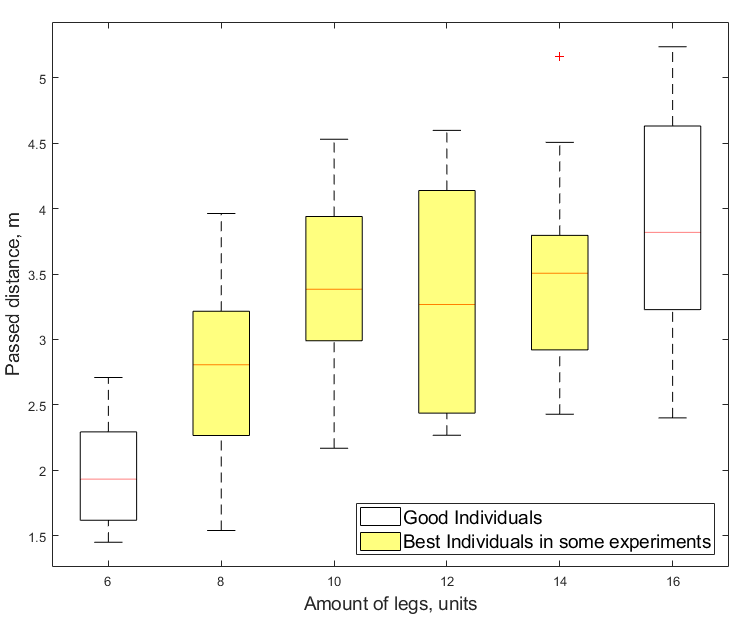
\includegraphics[height=4.5cm,width=1\textwidth,keepaspectratio]{images/box_plot_structural_synthesis.png}
    \caption{Зависимость между количеством ног и пройденной дистанцией}
    \label{fig:box_plot_structural_synthesis.png}
\end{figure}

Этот факт может быть объяснён следующими соображениями. С одной стороны, слишком много ног значительно удлиняет корпус робота, что снижает его профильную проходимость за счёт того, что робот с большей вероятностью может задеть выступы при движении. С другой стороны при слишком малом количестве ног происходит потеря статической устойчивости робота. Поскольку для гарантированного обеспечения статической устойчивости необходимо обеспечить контакт не менее, чем 4 ног с опорной поверхностью в каждый момент времени, то естественным ограничением является 8 ног у робота.

\textbf{Вторая задача:} найти оптимальный угол между соседними ногами робота при прямолинейном движении, чтобы средний клиренс был максимально возможным, а колебания корпуса робота --- минимальны.

Задача целевой функции --- максимизировать положение $Z$ и минимизировать $STD$. Одновременно необходимо сделать минимальным среднеквадратичное значение ($RMS$) и среднее стандартное отклонение ($STD$) углов по направлениям тангажа и крена. Целевая функция учитывает направление движения.

Целевая функция выглядит следующим образом:
\begin{align}
    \label{eq:objective}
    F = \sum\limits_{i=1}^4 \omega_{i} \cdot (\frac{1}{\omega_{z1}Z_{rms}^i - \omega_{z2}Z_{std}^i}  + ( \omega_{p1}\alpha_{rms}^i + \omega_{p2}\alpha_{std}^i) + \nonumber \\\ + (\omega_{r1}\beta_{rms}^i + \omega_{r2}\beta_{std}^i)) \rightarrow min
\end{align}
где $i =\{1,2,3,4\}$ индекс, который определяет направление движения: 1 --- вперед, 2 --- влево, 3 --- вправо, 4 --- вращение; $Z$ координата по оси Z; $\alpha, \beta$ значения ориентации по крену и тангажу; $\omega_{i}$ весовой коэффициент для направления движения, ${\omega}_{z,roll,pitch}$ весовые коэффициенты.

Решение задачи оптимизации проводилась с помощью метода полного перебора из-за проверки всего 2073600 вариантов.

\textbf{Третья задача:} разработать концепт корпуса робота для максимизации курсовой проходимости, без изменения длинны ног робота.

\begin{figure}[H]
    \centering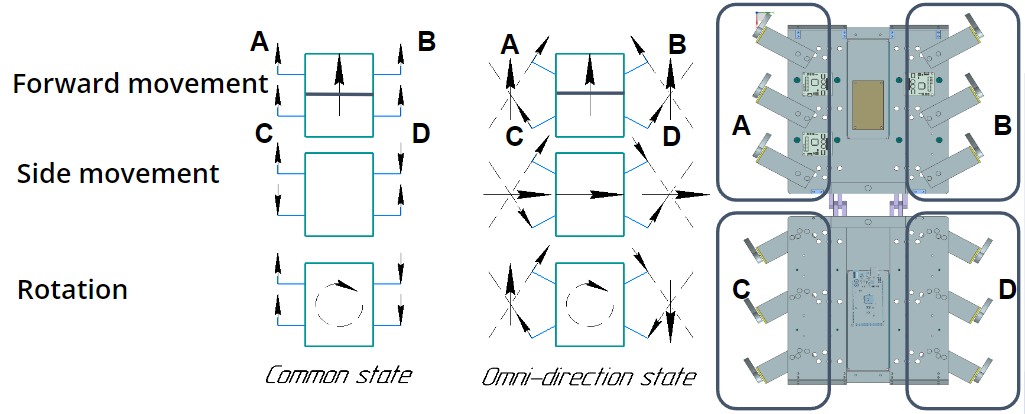
\includegraphics[height=3.5cm,width=1\textwidth,keepaspectratio]{omni_rot.png}
    \caption{Векторное представление сил в классическом и всенаправленном состоянии}
    \label{fig:omnidirection}
\end{figure}

\begin{figure}[H]
    \centerfloat{
        \hfill
        \subcaptionbox[List-of-Figures entry]{Первая итерация\label{fig:strirus_0}}{%
            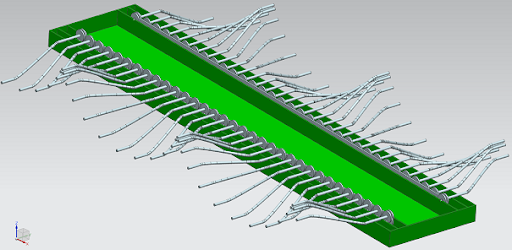
\includegraphics[width=0.33\linewidth]{strirus_0.png}}
        \hfill
        \subcaptionbox[List-of-Figures entry]{Вторая итерация \label{fig:strirus_1}}{%
            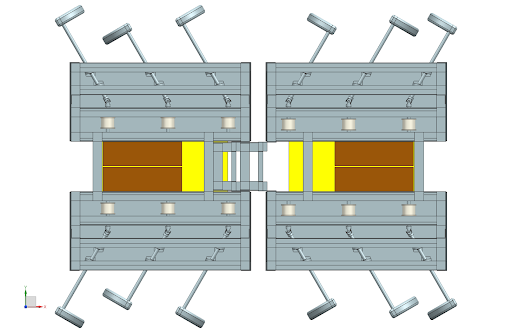
\includegraphics[width=0.33\linewidth]{strirus_1.png}}
        \hfill
        \subcaptionbox{Третья итерация\label{fig:strirus_2}}{%
        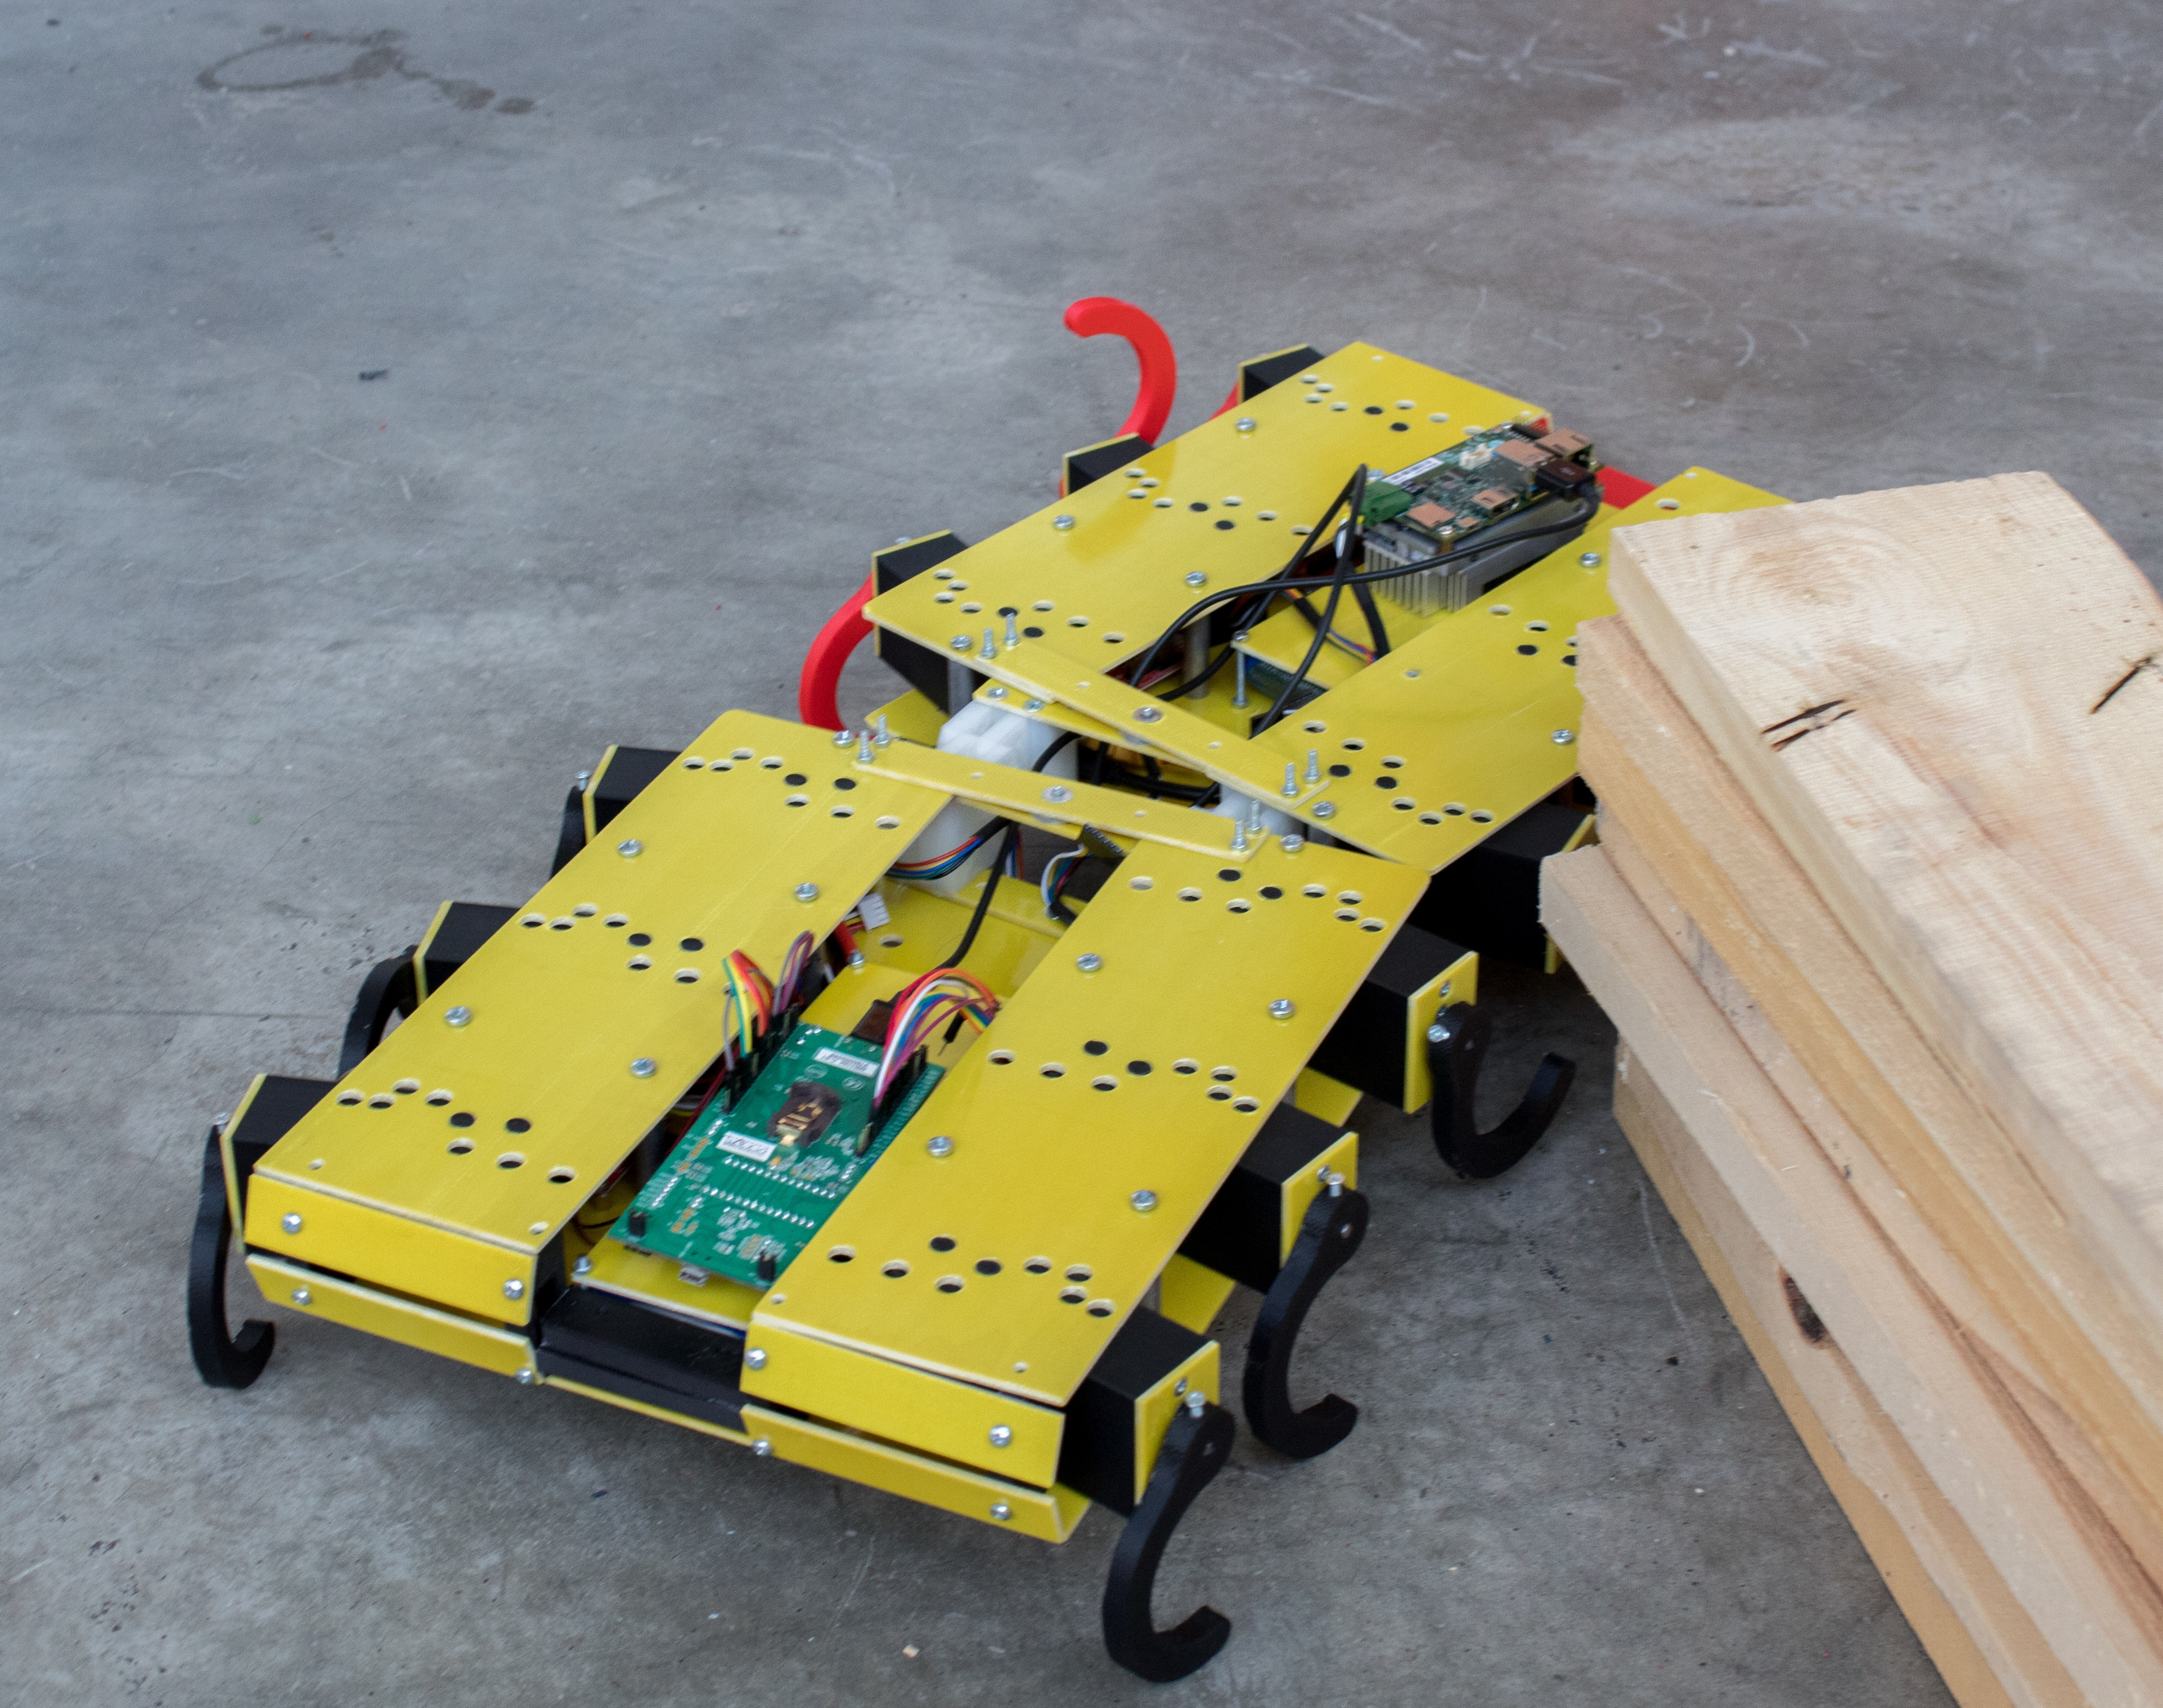
\includegraphics[width=0.33\linewidth]{strirus_2.jpg}}
        \hfill
        \subcaptionbox{Третья итерация +\label{fig:strirus_3}}{%
        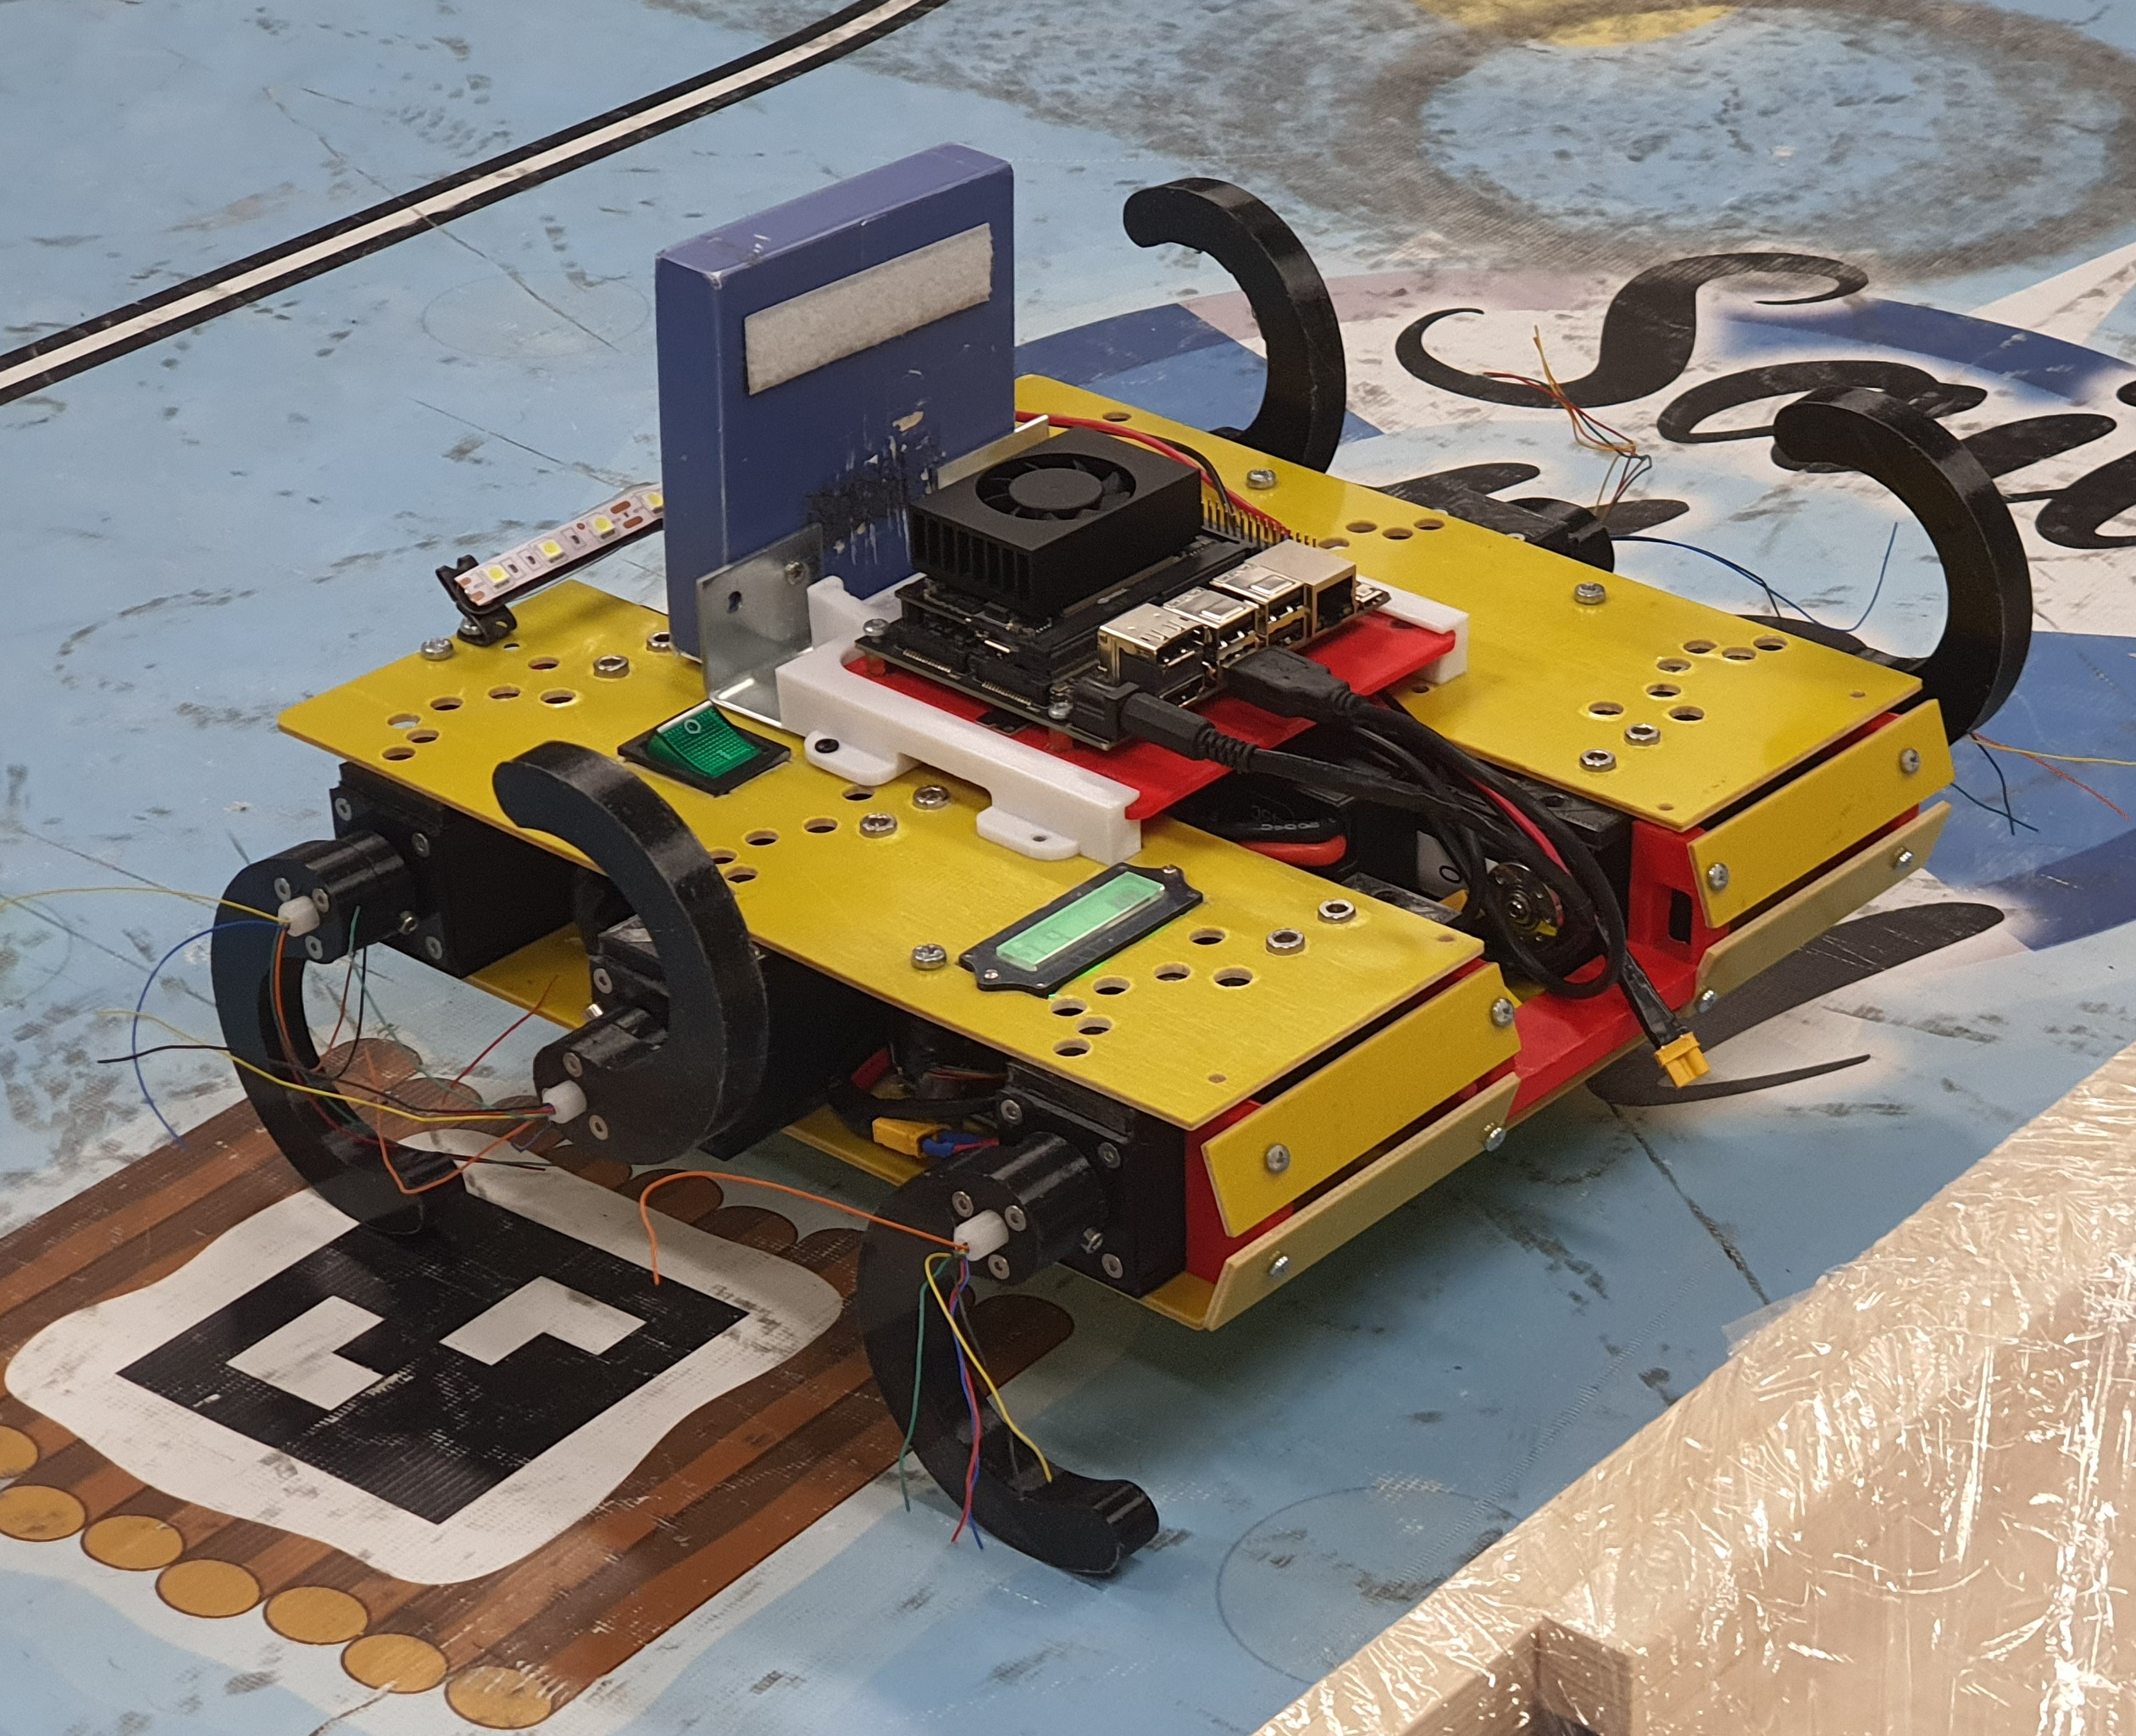
\includegraphics[width=0.35\linewidth]{strirus_3.JPG}}
        \hfill
        \subcaptionbox{Четвертая итерация\label{fig:strirus_4}}{%
        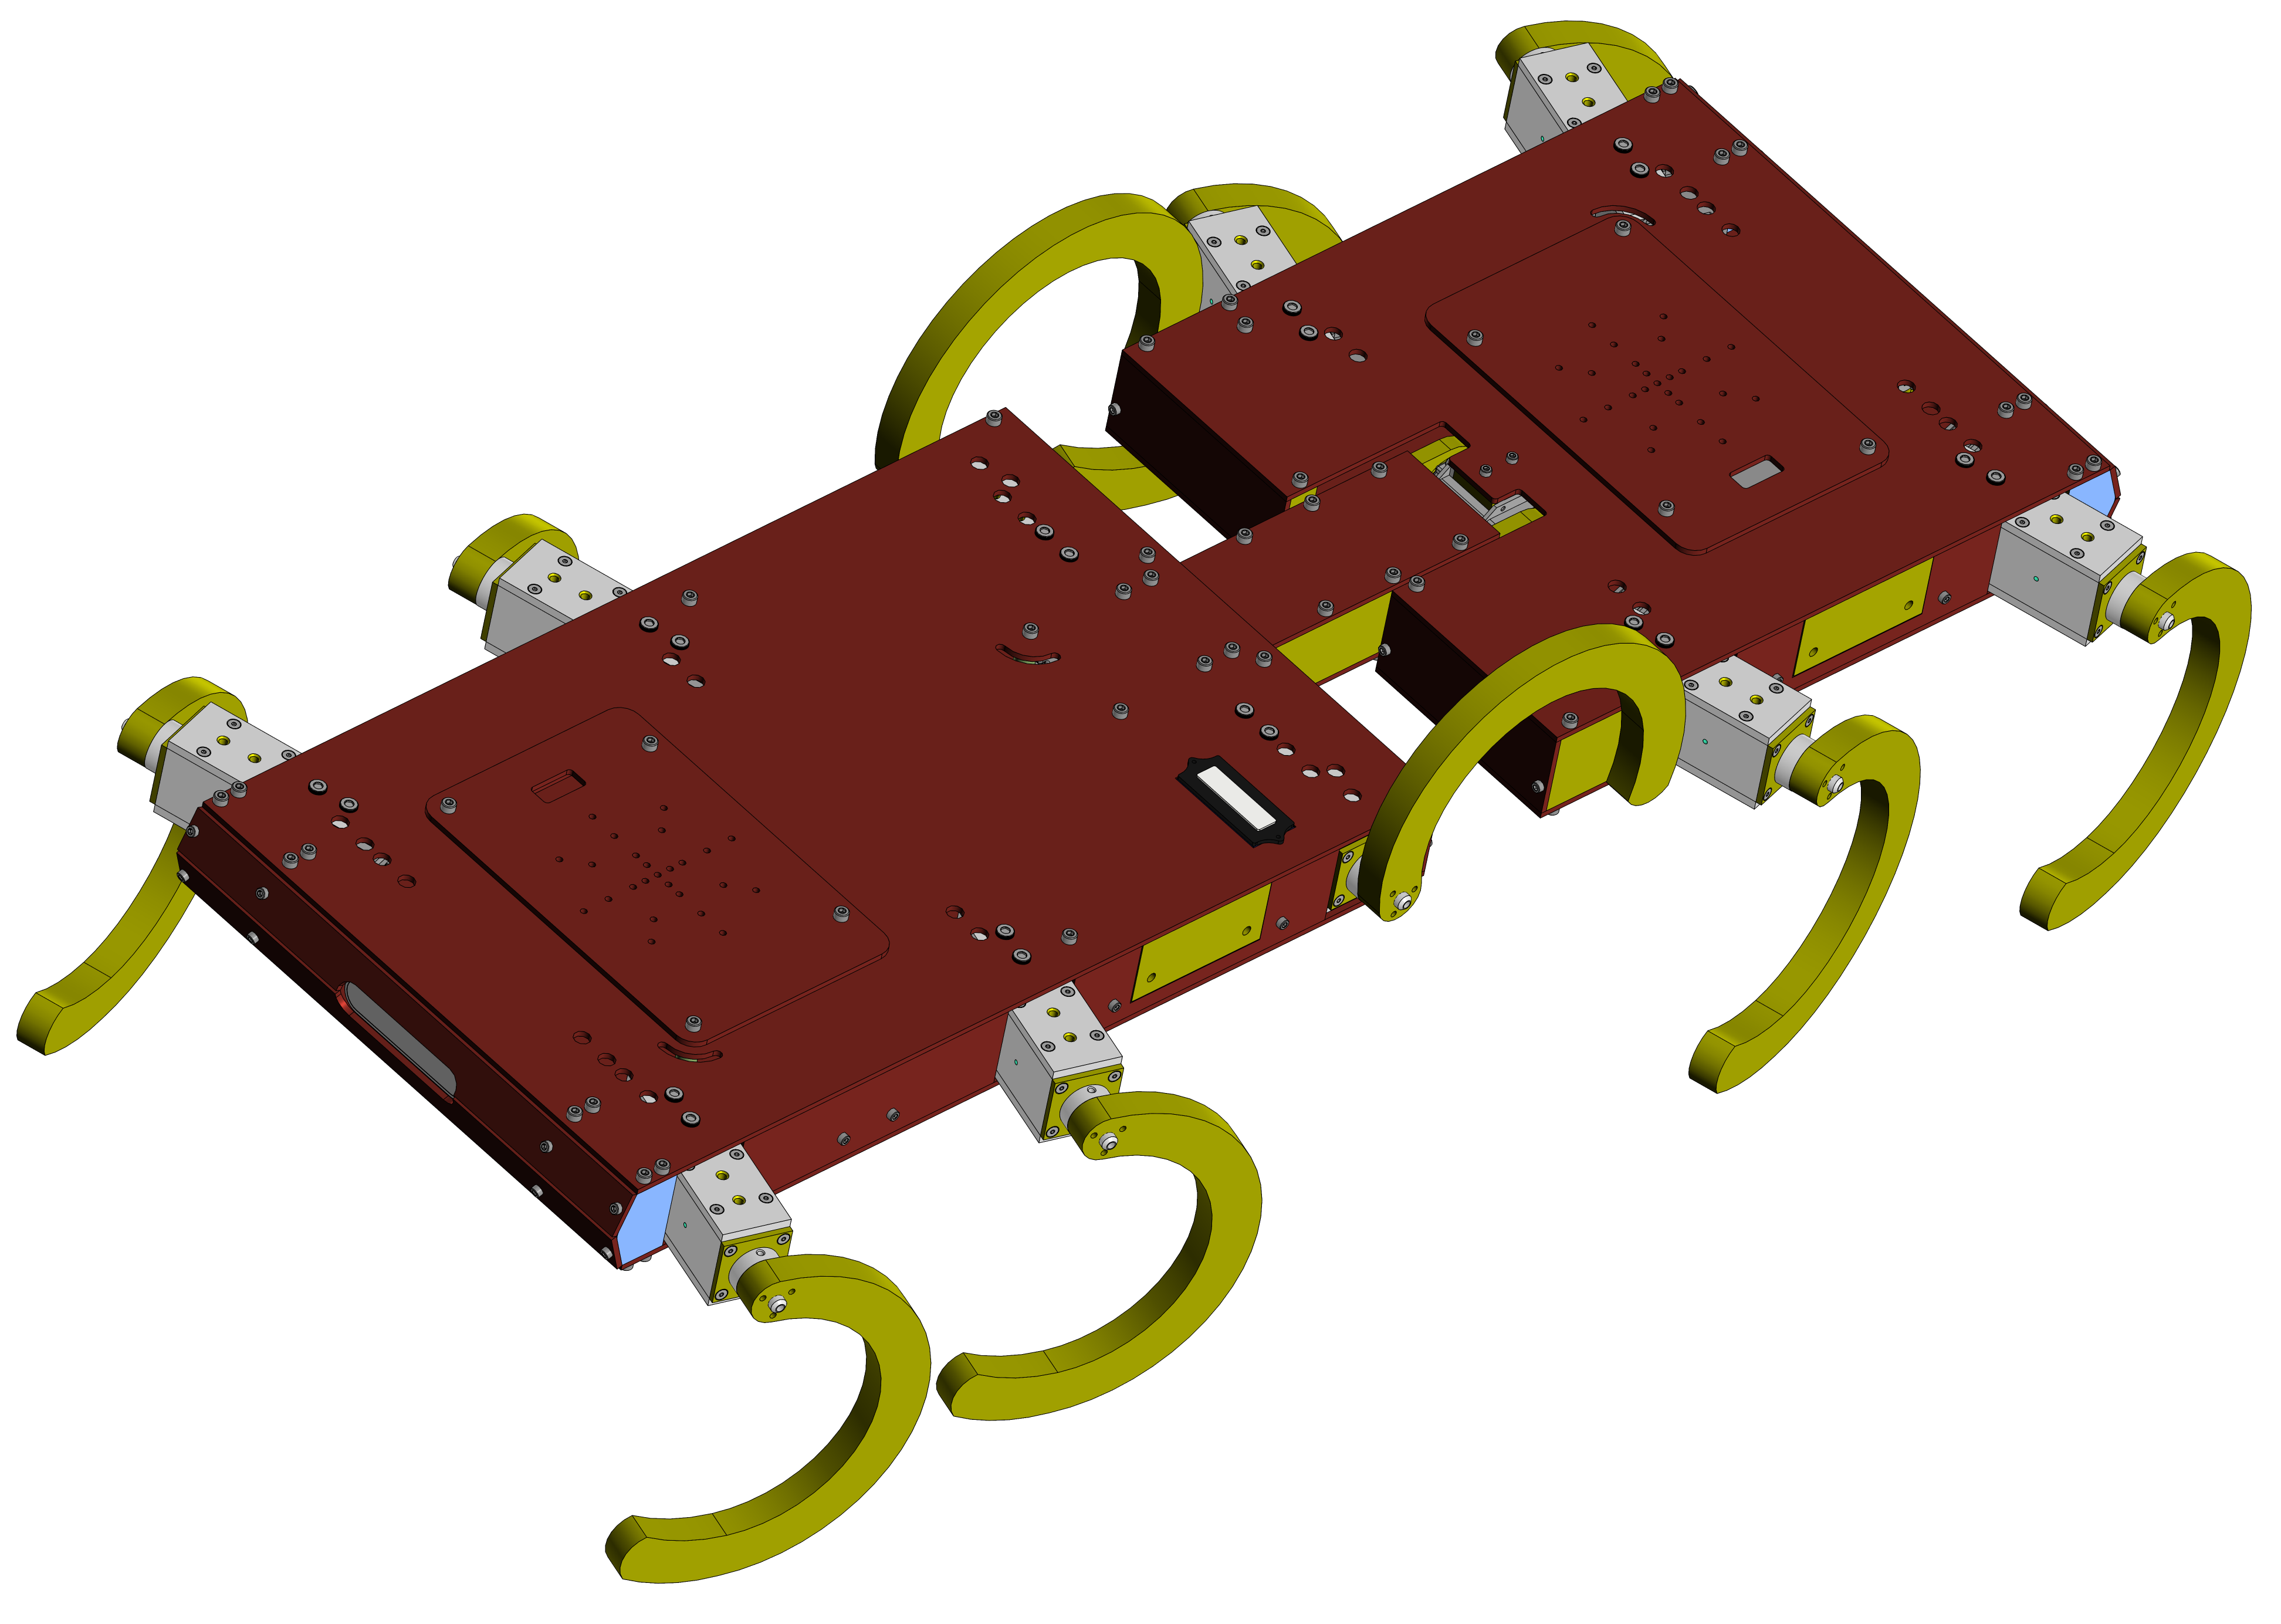
\includegraphics[width=0.35\linewidth]{strirus_4.png}}
    }
    \caption{Итерации робота СтриРуса}\label{fig:striruses}
  \end{figure}

На рисунке \ref{fig:omnidirection} представлена иллюстрация данной концепции: для того, чтобы робот двигался во всех направлениях, необходимо разбить ноги на группы, чтобы получилось 4 группы A-D и сделать так, чтобы угол между корпусом робота и осью вала привода ноги не было равен 90 градусам.
 Стрелка в центре робота — суперпозиция всех сил. Если изменить угол оси привода ноги в соответствии с предлагаемой концепцией, то возможно получить значения суперпозиции сил, представленные на рис. \ref{fig:omnidirection} в центре. То есть, чтобы переместить корпус робота направо, группы А и D должны вращать ноги в одну сторону, а группы C и B — в противоположную. Правая часть рисунка иллюстрирует расположение групп ног на исследуемом роботе. 

В рамках работы было разработано четыре концепции робота СтриРус \pic{fig:striruses}. Видео 4ой итерации \quad \qrcode[height=1.5cm]{https://youtu.be/EQ6oGZVDpoc}


Как итог, был разработан десятиногий двух сегментный робот СтриРус. 10 ног было выбрано на основе результатов, полученных во время решения мультикритериальной задачи оптимизации с помощью генетического алгоритма.


